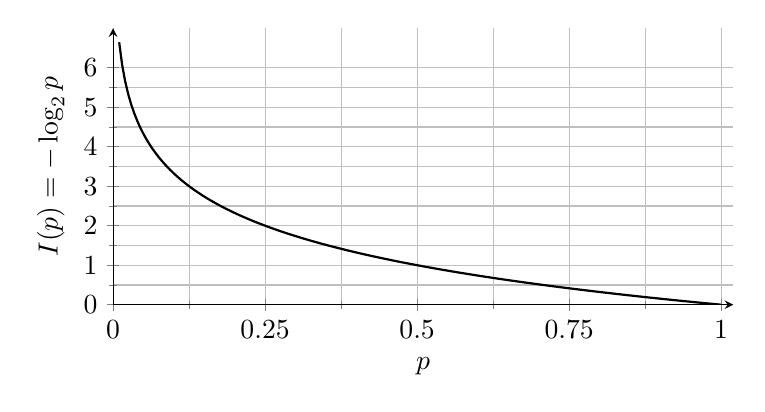
\begin{tikzpicture}
  \begin{axis}[
    width=0.78\textwidth,
    height=0.42\textwidth,
    domain=0.01:1,
    samples=200,
    axis lines=left,
    xmin=0, xmax=1.02,
    ymin=0, ymax=7,
    xlabel={$p$},
    ylabel={$I(p)=-\log_2 p$},
    xtick={0,0.25,0.5,0.75,1},
    ytick={0,1,2,3,4,5,6},
    grid=both,
    minor tick num=1,
  ]
    \addplot[thick] {-ln(x)/ln(2)};
  \end{axis}
\end{tikzpicture}